\documentclass[12pt]{article}
\usepackage{geometry}                % See geometry.pdf to learn the layout options. There are lots.
\geometry{letterpaper}                   % ... or a4paper or a5paper or ... 
%\geometry{landscape}                % Activate for for rotated page geometry
\usepackage[parfill]{parskip}    % Activate to begin paragraphs with an empty line rather than an indent
\usepackage{daves,fancyhdr,natbib,graphicx,dcolumn,amsmath,lastpage,url}
\usepackage{amsmath,amssymb,epstopdf,longtable}
\usepackage{paralist}  % need to properly formulate standard answer blocks
\DeclareGraphicsRule{.tif}{png}{.png}{`convert #1 `dirname #1`/`basename #1 .tif`.png}
\pagestyle{fancy}
\lhead{CE 3305 Fluid Mechanics}
\rhead{Name:\_\_\_\_\_\_\_\_\_\_\_\_\_\_\_\_\_\_\_\_\_\_\_\_\_\_\_\_\_\_\_\_\_\_}
\lfoot{REVISION B}
\cfoot{}
\rfoot{Page \thepage\ of \pageref{LastPage}}
\renewcommand\headrulewidth{0pt}



\begin{document}
\begingroup
\begin{center}
{\textbf{{ CE 3305 Fluid Mechanics} \\ Exercise Set 18 \\ Summer 2018 -- GERMANY } }
\end{center}
\endgroup

%%%%%%%%%%%%%%%%%%%%%%%%%%%
%\begin{enumerate}
%%%%%%%%%%%%%%%%%%%%%%%%%%%%%%%%%
 The pressure drop over 150 m of 10-cm-diameter galvanized iron pipe is measured to be 100 kPa.  
Roughness height is $k_s = 0.2 0$ millimeters.  
If the pipe is horizontal, estimate the flow rate of water.  
Express the result in Liters per second.  ($\nu = 10^{-6} m^2/sec$)

\begin{figure}[h!] %  figure placement: here, top, bottom, or page
   \centering
   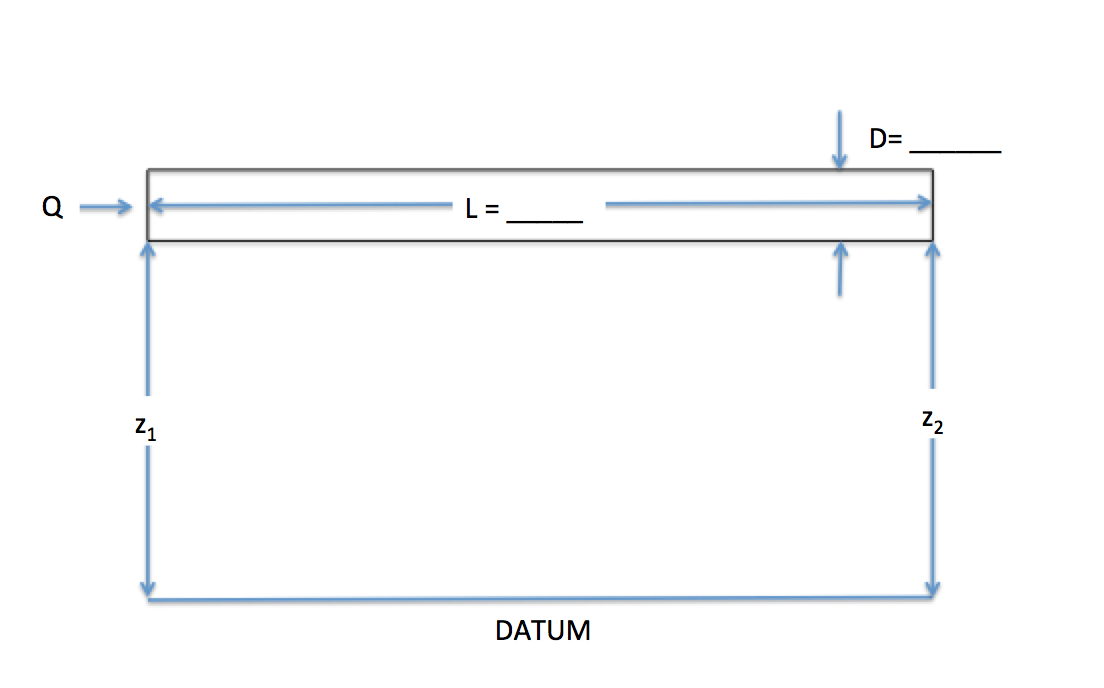
\includegraphics[width=5in]{PipelineSketch.jpg} 
   \caption{Problem Sketch}
   \label{fig:PipelineSketch}
\end{figure}

\begin{enumerate}[a)]
\item Write the pipe length on the sketch depicted in Figure \ref{fig:PipelineSketch}, include units.
\item Write the pipe diameter on the sketch depicted in Figure \ref{fig:PipelineSketch}, include units.
\item Horizontal means (circle correct response)\\
$z_1 > z_2$ \\
$z_1 = z_2$ \\
$z_1 < z_2$ 
\item Constant diameter pipe means (circle correct response)\\
$V_1 > V_2$ \\
$V_1 = V_2$ \\
$V_1 < V_2$ 
\newpage
The energy equation for this pipeline is\\~\\
$ \frac{p_1}{\rho g} + \frac{V_1^2}{2g} + z_1= \frac{p_2}{\rho g} + \frac{V_1^2}{2g} +z_2 + f\frac{L}{D}\frac{V^2}{2g}$\\~\\
\item Cancel the terms that are identical because the pipeline is horizontal.
\item Cancel the terms that are identical because the pipeline is constant diameter.
\item Compute the relative roughness \\~\\
\begin{math}
  \frac{k_s}{D} = 
\end{math} 
\\
\item Highlight the appropriate relative roughness curve on the Moody chart on Figure \ref{fig:Moody Chart}.
\begin{figure}[h!] %  figure placement: here, top, bottom, or page
\centering
   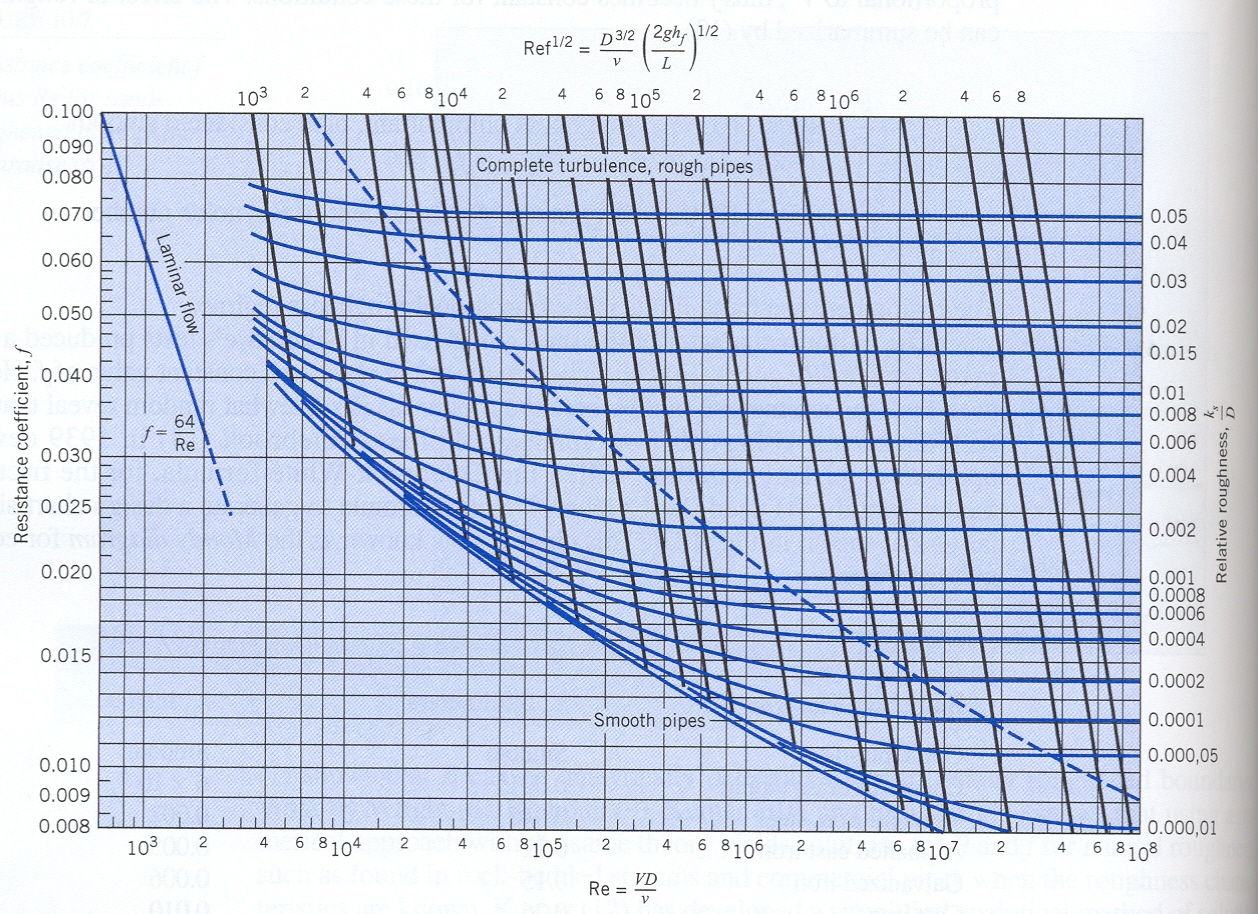
\includegraphics[width=6in]{Moody.jpg}
   \caption{Moody Chart for Problem 1}
   \label{fig:Moody Chart} 
\end{figure}
\item For Reynolds number larger than $10^5$ what is the value of the friction factor $f$?\\
\item Rearrange the remaining terms of the energy equation to equate the difference in pressure head to the head loss equation.\\~\\~\\
\item Compute the numerical value of change in pressure head, in meters?\\~\\~\\
\item What is the velocity in the pipe for the given change in pressure head assuming relatively high Reynolds number?\\~\\~\\
\item What is the Reynolds number for this velocity?\\~\\~\\
\item Plot the intersection of the computed Reynolds number and the relative roughness on the Moody chart.\\
\item Is the initial guess of friction factor reasonable based on the plot?\\
\item Compute the discharge in the pipe in liters per second.
\end{enumerate}
%\end{enumerate}






%\clearpage
%(Quiz 5) (Continued)

\end{document}  